\documentclass[12pt]{article}
\usepackage{graphicx}
\usepackage{enumitem}
\usepackage{amsmath}
\usepackage{gvv-book}
\usepackage{gvv}
\title{\textbf{2.3.8}}
\author{\textbf{EE25BTECH11005 - Aditya Mishra}}
\date{September 12, 2025}
\begin{document}
\maketitle
\section*{Question}
If $ \vec{A} = \hat{i} + \hat{j} + \hat{k},\ \vec{B} = 2\hat{i} + 5\hat{j},\ \vec{C} = 3\hat{i} + 2\hat{j} - 3\hat{k},\ \vec{D} = \hat{i} - 6\hat{j} - \hat{k}$ are the position vectors of points A, B, C and D, then find the angle between the straight lines $AB$ and $CD$. Find whether $(\vec{B}-\vec{A})$ and $(\vec{D}-\vec{C})$ are collinear or not.

\section*{Solution}
The direction vectors are
\begin{align}
\vec{B} - \vec{A} &= \myvec{2\\5\\0} - \myvec{1\\1\\1} = \myvec{1\\4\\-1} \\
\vec{D} - \vec{C} &= \myvec{1\\-6\\-1} - \myvec{3\\2\\-3} = \myvec{-2\\-8\\2}
\end{align}

The angle $\theta$ between $\vec{B}-\vec{A}$ and $\vec{D}-\vec{C}$ is
\begin{align}
\cos\theta = \frac{(\vec{B}-\vec{A})^\top (\vec{D}-\vec{C})}{\|\vec{B}-\vec{A}\|\,\|\vec{D}-\vec{C}\|}
\end{align}

Substitute:
\begin{align}
(\vec{B}-\vec{A})^\top(\vec{D}-\vec{C}) &= \myvec{1 & 4 & -1}\myvec{-2\\-8\\2} \\
&= -2 - 32 - 2 = -36
\end{align}

Magnitudes:
\begin{align}
\|\vec{B}-\vec{A}\| &= \sqrt{1^2+4^2+(-1)^2} = \sqrt{18} \\
\|\vec{D}-\vec{C}\| &= \sqrt{(-2)^2+(-8)^2+2^2} = \sqrt{72}
\end{align}

Thus,
\begin{align}
\cos\theta = \frac{-36}{\sqrt{18}\sqrt{72}} 
= \frac{-36}{36} = -1
\end{align}
\begin{align}
\theta = \cos^{-1}(-1) = \pi \ \text{radians} = 180^\circ
\end{align}

\subsection*{Collinearity using Rank}
For collinearity, consider the matrix
\begin{align}
M = \myvec{1 & 4 & -1 \\ -2 & -8 & 2}
\end{align}

If $\text{rank}(M)=1$, then the two vectors are linearly dependent (collinear).

Performing row reduction:
\begin{align}
M &= \myvec{1 & 4 & -1 \\ -2 & -8 & 2} \\
R_2 \to R_2 + 2R_1 &\implies \myvec{1 & 4 & -1 \\ 0 & 0 & 0}
\end{align}

Hence,
\begin{align}
\text{rank}(M) = 1
\end{align}

Therefore, $(\vec{B}-\vec{A})$ and $(\vec{D}-\vec{C})$ are collinear. Since $\theta = 180^\circ$, they are anti-parallel.

\begin{figure}[H]
    \centering
    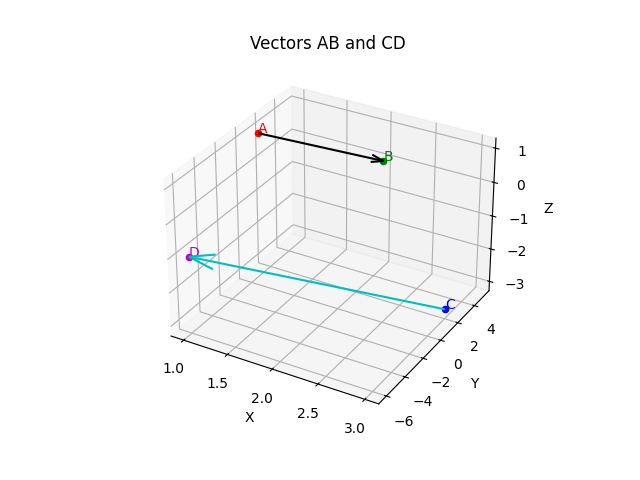
\includegraphics[width=0.7\columnwidth]{Figs/Figure.png}
    \caption{Line directions}
    \label{fig:ab_cd}
\end{figure}

\end{document}

